\documentclass[dvipsnames,beamer]{standalone}

\usepackage{tikz}
\usetikzlibrary{positioning,decorations.pathreplacing,fit}
\usetikzlibrary{decorations.markings,arrows.meta,shapes.arrows,arrows}
\usetikzlibrary{calc}

\definecolor{darkgreen}{RGB}{0,128,80}


\begin{document}

\begin{standaloneframe}

\resizebox{\textwidth}{!}{

\begin{tikzpicture}[
	arrow double line/.style={
		double distance = 20pt,
   		shorten <= 11, 	
   		shorten >= 16,
   		very thick,
	    postaction = {
    		draw = white,
	 	    line width = 20pt,
	 	    shorten <=-.1pt,
	 	    shorten >=-.1pt,	
	    },
	    postaction = {
	    	decorate, 
	    	decoration = {
	    		markings, 
	    		mark=at position 0 with {
	    			\arrow[xshift=26.6pt]{Straight Barb[reversed,length=-1pt 0.7]}
	    		},
	    		mark = at position 1 with {
   	    			\arrow[xshift=10.6pt]{Straight Barb[length=-1pt 0.7]}
   	    		}
	    	}
	    }
	},
	mysingle/.style = {
		double distance = 22,
		shorten <= 10.5, 	
		shorten >= 14,
		very thick,
		postaction = {
	 		draw = white,
			line width = 22pt,
			shorten <=8pt,
			shorten >=-.5pt,	
		},
		postaction = {
			decorate, 
			decoration = {
				markings, 
				mark = at position 1 with {
					\arrow [xshift=15]{Straight Barb[length=15]}
				}
			}
		},	
	},	
	mybrace/.style= {
		decorate, decoration={brace,amplitude=5pt,raise=5pt}, thick
	},
	every node/.style={
		font=\bfseries\boldmath
	},
	]

	\def\AtB{4.8}
	\def\BtT{4.0}
	\def\InterMsgSpaceVertical{1}
	
	
	\node[align=center] (client) {\large C};
	\node[above=-0.2 of client] (foo) {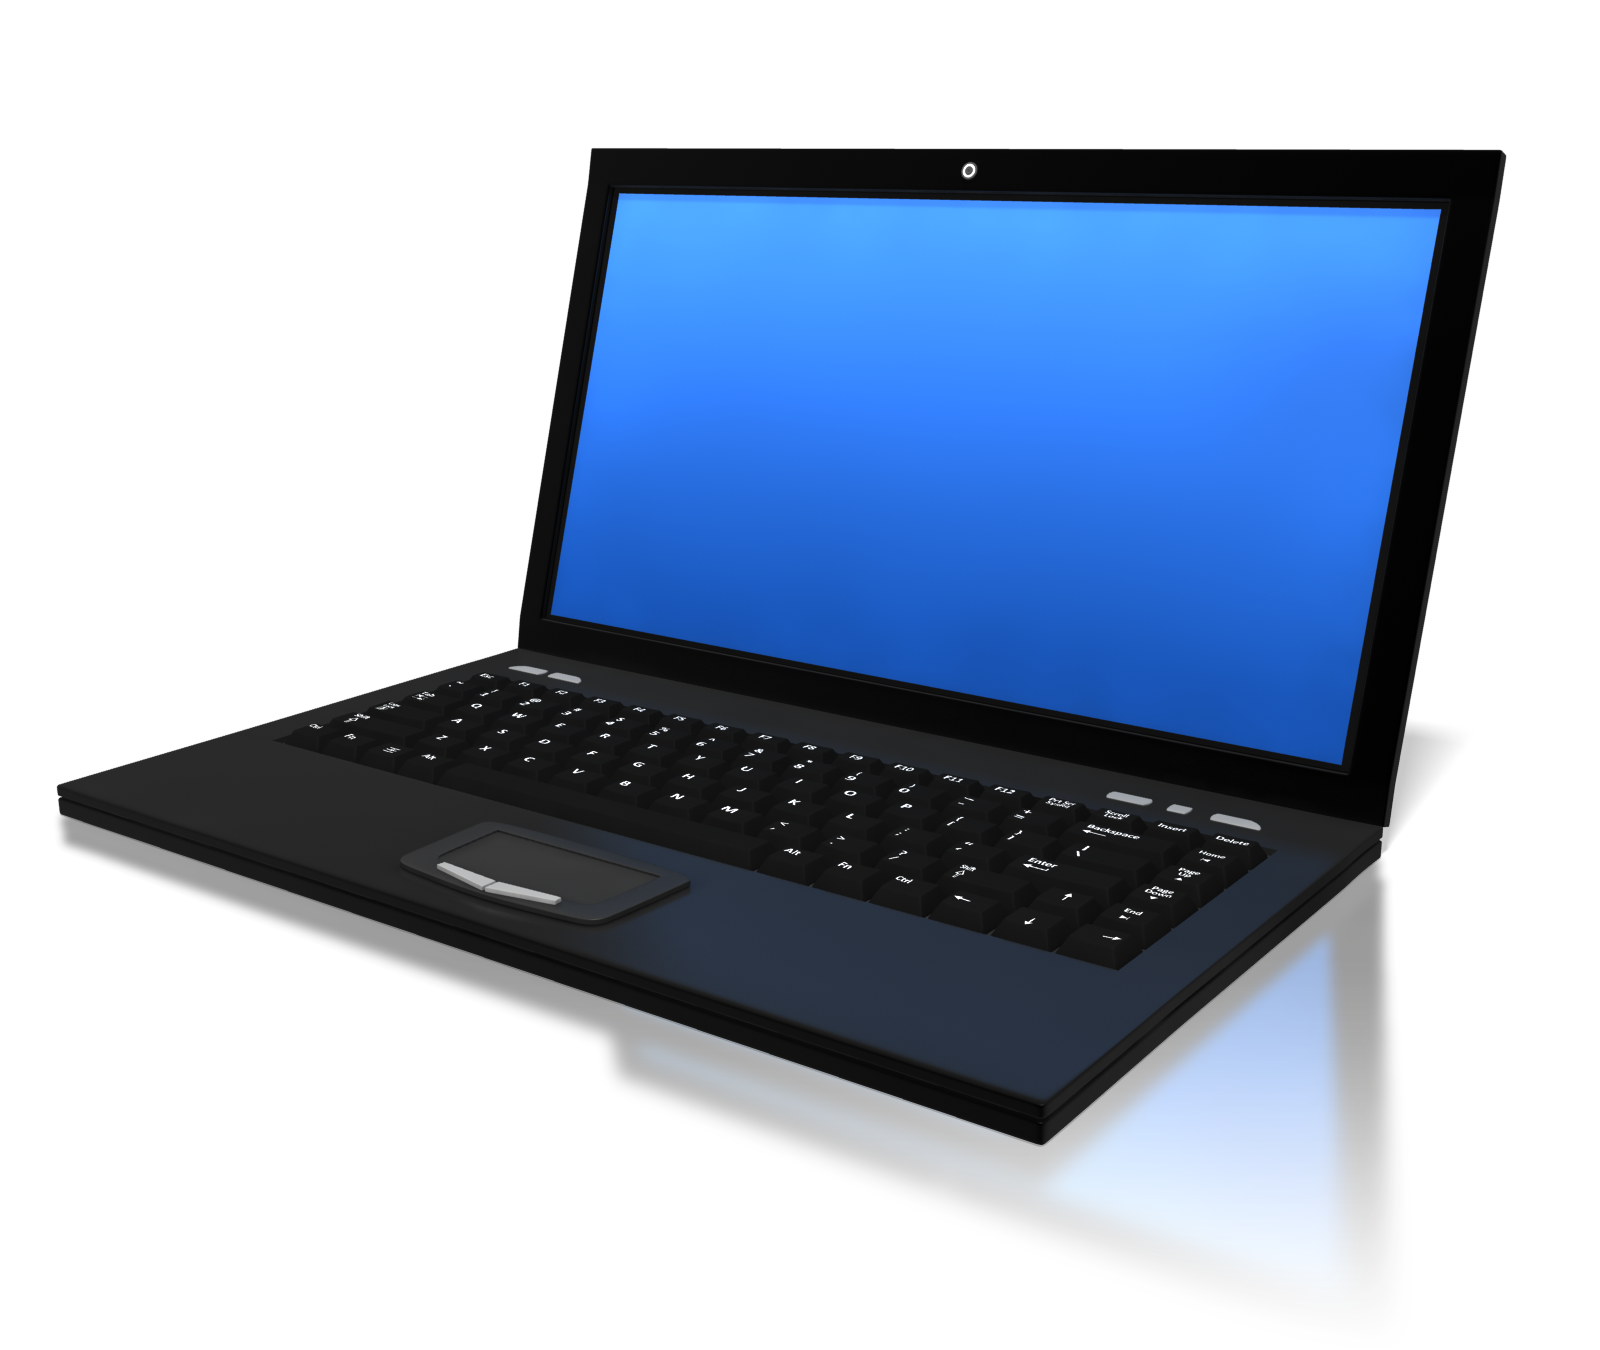
\includegraphics[width=.15\textwidth]{laptop}};
	
	\node[right = \AtB of client,align=center] (AP) {\large A};
	\node[above = 0 of AP] () {
\includegraphics[width=.13\textwidth]{AP}};
	
	\node[right = \BtT of AP.east,align=center] (AS) {\large S};
	\node[above = -0.2 of AS] () {
\includegraphics[width=.1\textwidth]{server}};
	
	\foreach \i in {1,...,8} {
		\coordinate[below = \InterMsgSpaceVertical * (\i-1) of client] (c\i) {};
		\coordinate[below = \InterMsgSpaceVertical * (\i-1) of AP] (ap\i) {};
		\coordinate[below = \InterMsgSpaceVertical * (\i-1) of AS] (as\i) {};
	}
	

	\draw[arrow double line, Plum] (c2) -- node {$\Pi_3$ (3P-AKE$^w$)} (as2);
	
	\draw[mysingle, Plum] ([yshift=0]ap2) --  ([yshift=-10.5]ap3);
	
	\visible<1->{
		\draw[arrow double line,darkgreen] (c4) -- node[xshift=0] {
			$\Pi_4$ (2P-AKE$^\mathsf{static}$ + EA)
		} (ap4);
	}
	
	\visible<1->{
		\draw[mybrace, decoration={mirror}, left] ([xshift=-0.5cm,yshift=13]c2) -- node[left=0.4,align=center] {$\Pi_5$} ([xshift=-0.5cm,yshift=-13]c4);
%		\draw[mybrace mirror, left] ([xshift=-0.5cm,yshift=8]c2) -- node[left=0.4,align=center] {$\Pi_5$\\(3P-AKE)} ([xshift=-0.5cm,yshift=-8]c4);
	}

	

\end{tikzpicture}

}

\end{standaloneframe}

\end{document}